\documentclass[a4paper,11pt]{article}
\usepackage{amsmath,amsthm,amsfonts,amssymb,amscd,amstext,vmargin,graphics,graphicx,tabularx,multicol} 
\usepackage[francais]{babel}
\usepackage[utf8]{inputenc}  
\usepackage[T1]{fontenc} 
\usepackage{pstricks-add,tikz,tkz-tab,variations}
\usepackage[autolanguage,np]{numprint} 

\setmarginsrb{1.5cm}{0.5cm}{1cm}{0.5cm}{0cm}{0cm}{0cm}{0cm} %Gauche, haut, droite, haut
\newcounter{numexo}
\newcommand{\exo}[1]{\stepcounter{numexo}\noindent{\bf Exercice~\thenumexo} : \marginpar{\hfill /#1}}
\reversemarginpar


\newcounter{enumtabi}
\newcounter{enumtaba}
\newcommand{\q}{\stepcounter{enumtabi} \theenumtabi.  }
\newcommand{\qa}{\stepcounter{enumtaba} (\alph{enumtaba}) }
\newcommand{\initq}{\setcounter{enumtabi}{0}}
\newcommand{\initqa}{\setcounter{enumtaba}{0}}

\newcommand{\be}{\begin{enumerate}}
\newcommand{\ee}{\end{enumerate}}
\newcommand{\bi}{\begin{itemize}}
\newcommand{\ei}{\end{itemize}}
\newcommand{\bp}{\begin{pspicture*}}
\newcommand{\ep}{\end{pspicture*}}
\newcommand{\bt}{\begin{tabular}}
\newcommand{\et}{\end{tabular}}
\renewcommand{\tabularxcolumn}[1]{>{\centering}m{#1}} %(colonne m{} centrée, au lieu de p par défault) 
\newcommand{\tnl}{\tabularnewline}

\newcommand{\bmul}[1]{\begin{multicols}{#1}}
\newcommand{\emul}{\end{multicols}}

\newcommand{\trait}{\noindent \rule{\linewidth}{0.2mm}}
\newcommand{\hs}[1]{\hspace{#1}}
\newcommand{\vs}[1]{\vspace{#1}}

\newcommand{\N}{\mathbb{N}}
\newcommand{\Z}{\mathbb{Z}}
\newcommand{\R}{\mathbb{R}}
\newcommand{\C}{\mathbb{C}}
\newcommand{\Dcal}{\mathcal{D}}
\newcommand{\Ccal}{\mathcal{C}}
\newcommand{\mc}{\mathcal}

\newcommand{\vect}[1]{\overrightarrow{#1}}
\newcommand{\ds}{\displaystyle}
\newcommand{\eq}{\quad \Leftrightarrow \quad}
\newcommand{\vecti}{\vec{\imath}}
\newcommand{\vectj}{\vec{\jmath}}
\newcommand{\Oij}{(O;\vec{\imath}, \vec{\jmath})}
\newcommand{\OIJ}{(O;I,J)}


\newcommand{\reponse}[1][1]{%
\multido{}{#1}{\makebox[\linewidth]{\rule[0pt]{0pt}{20pt}\dotfill}
}}

\newcommand{\titre}[5] 
% #1: titre #2: haut gauche #3: bas gauche #4: haut droite #5: bas droite
{
\noindent #2 \hfill #4 \\
#3 \hfill #5

\vspace{-1.6cm}

\begin{center}\rule{6cm}{0.5mm}\end{center}
\vspace{0.2cm}
\begin{center}{\large{\textbf{#1}}}\end{center}
\begin{center}\rule{6cm}{0.5mm}\end{center}
}



\begin{document}
\pagestyle{empty}
\titre{Contrôle - Division décimale et périmètre }{Nom :}{Prénom :}{Classe}{Date}

\vspace*{0.35cm}


\exo{4} Calculer le périmètre de la figure suivante :\\
\vspace*{-0.25cm}
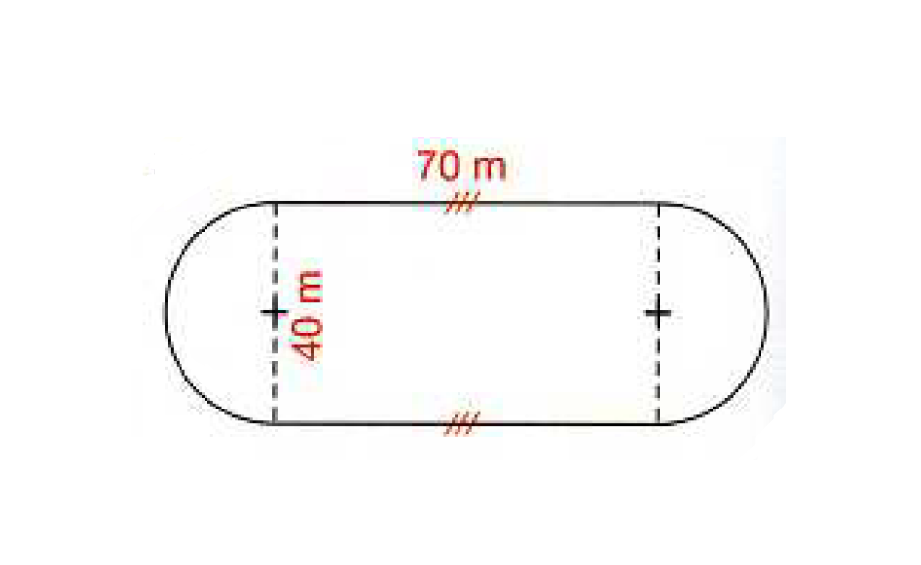
\includegraphics[scale=0.6]{perimetreccomplexe1.eps} 

\vspace*{0.35cm}

\exo{4} Poser et donner  \textbf{la valeur approchée} au millième près des divisions suivantes :
\bmul{3}

\qa 393 $\div$ 24\\


\columnbreak


\qa $904,3 \div 11$\\

\columnbreak

\qa $25,84 \div 1,2$\\

\emul

\vspace*{0.35cm}

\exo{4} \textbf{Les questions suivantes sont indépendantes.}\\

\initqa
\qa Gérard a payé 28,56 euros pour 12 pieds de tomates. Quel est le prix d'un pied de tomate ?\\

\qa Bastien a économisé tout son argent de poche de cette année. Ses parents lui ont donné la même somme d'argent tous les mois. Cela représente une somme de 480 euros.\\
 Combien d'argent ses parents lui donnait tous les mois ? \\
 
 \qa 6 amis se partagent au goûter une bouteille de 1,5L de soda. Combien de litre de soda boiront-ils chacun ?\\

\vspace*{0.35cm}

\exo{4}
Mélissa dispose de 20 euros. Elle achète 3 cahiers identiques et 8 stylos de couleur. \\
	Chaque stylo coûte  1,25 euros . La caissière lui rend 2,80 euros.\\
	 Quel est le prix d’un cahier ?\\

\vspace*{0.35cm}

\exo{4} Voici les tarifs pour le mensuel Mepmagazine :\\
- si on achète en magasin un numéro par mois à la fin de l'année, on aura payé 99 euros (soit 12 numéros);\\
- si on prend un abonnement, les 12 numéros coûtent 63 euros et les 24 numéros coûtent 114 euros.\\

\noindent \q Donner le prix d'un magazine si on l'achète en kiosque.\\
\q Donner le prix d'un magazine si on s'abonne pour 12 numéros.\\
\q Donner le prix d'un magazine si on s'abonne pour 24 numéros.\\
\q Quelle est la solution la plus avantageuse?\\

\vspace*{0.35cm}

\exo{} BONUS

Sur une planète, où poussent des fleurs immenses, un amoureux en cueille une
dont la corolle a 258 839 pétales !\\

Il commence à l’effeuiller et il dit « Elle m'aime » en enlevant le premier pétale, « un peu » en enlevant
le second, « beaucoup » en enlevant le troisième, puis « passionnément », « à la folie », « pas du
tout ». \\
Et il recommence : « Elle m'aime », « un peu », « beaucoup »...\\
\textbf{Quel va-t-il dire en effeuillant le dernier pétale ? Justifie ta réponse.}








\end{document}
